\chapter{Data}

\section{Data Acquisition}

This research project utilises the most recent open access spectral data from the GALAH survey. At the time of writing, the GALAH survey is in its third data release (GALAH DR3). DR3 comprises 678,423 spectra for 588,571 stars, of which approximately 80\% of these stars are within a radius of 2 kpc \cite{buder2021galah+}. Of the 588,571 stars, continuum normalised spectra of 588,343 have been provided.The GALAH DR3 (hereafter DR3) is accessible via the \href{https://www.galah-survey.org/}{survey website} and \href{https://datacentral.org.au/}{AAO Data Central}.

The data is organised as individual \texttt{.fits} format files. Each file contains an object ID prefix (known as an "\texttt{sobject\_id}") followed the last digit in the filename which serves as the camera number suffix. Thus, the file \texttt{1705090057010093.fits} is a data file for an object with \texttt{sobject\_id=170509005701009} and contains spectral data from camera 3 (or the red camera). The blue, green and infra red cameras are denoted by the suffix 1,2 and 4 respectively.
The red camera of the HERMES spectrograph is the spectral channel with the range 6478\r{A} - 6737\r{A}\cite{sheinis2014first}. This range is of particular interest to this research as the characteristic H$\alpha$ line appears within this range. These individual files totalling 385 GB were downloaded to a Macquarie University file server and served as the data source for all research and analytical work presented in this thesis.

\begin{figure}[h]
\centering
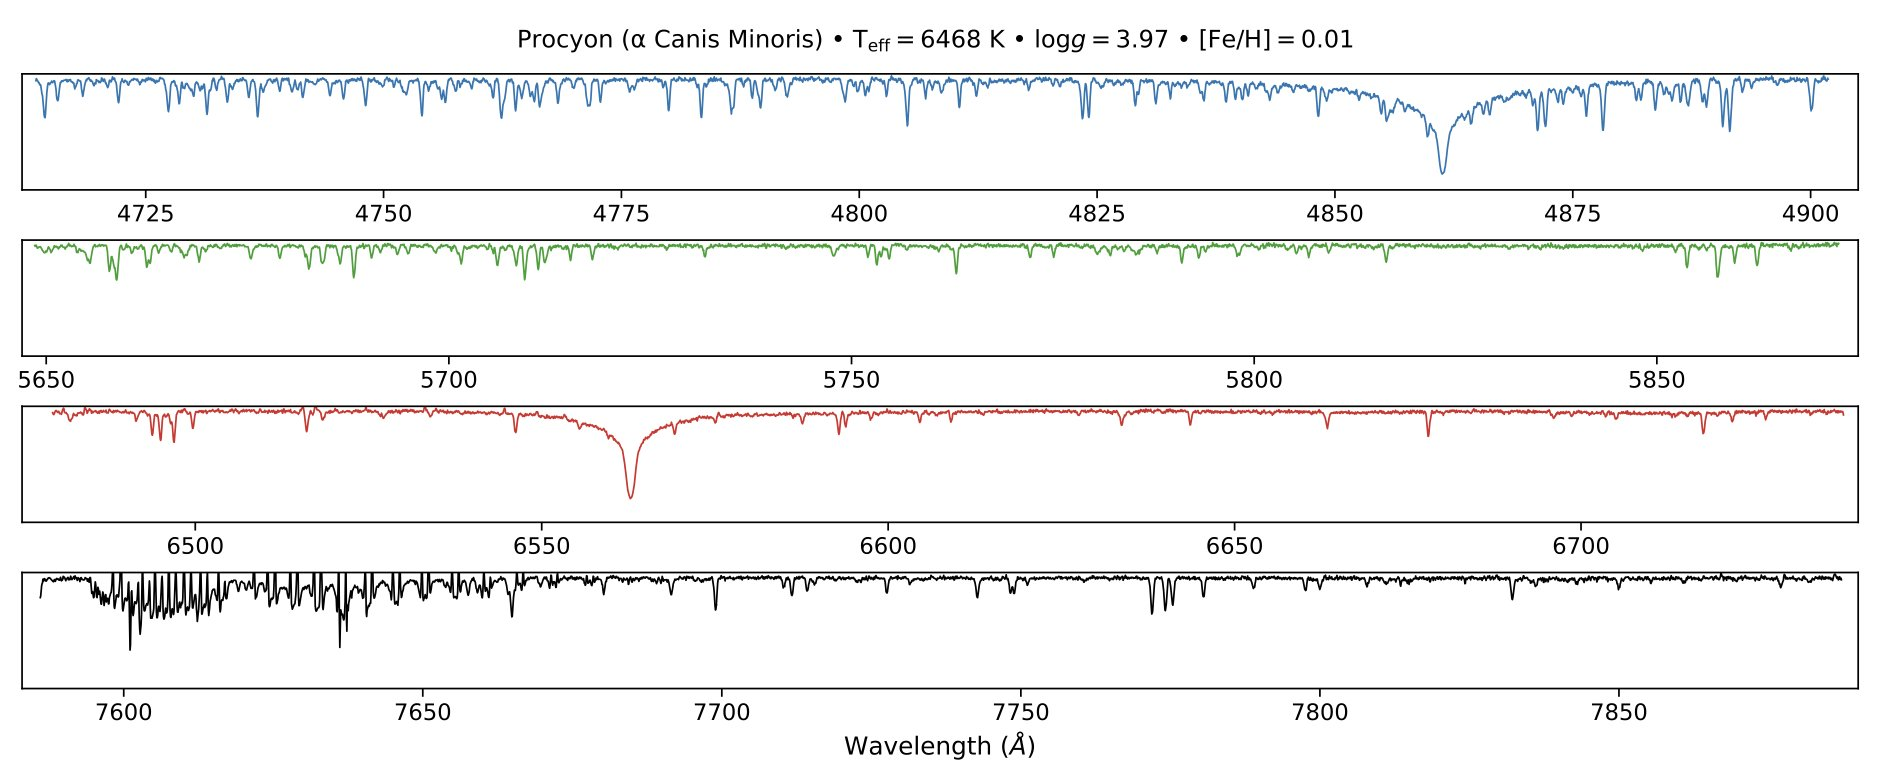
\includegraphics[scale=.25]{figures/galah cameras.jpeg}
\caption{Normalised spectral data for the star $\alpha$ Canis Minoris. Figure \cite{kasai2013type}}
\end{figure}

Čotar et al. used DR3\cite{de2015galah}, the K2-HERMES survey\cite{wittenmyer2018k2} and the TESS-HERMES survey\cite{sharma2018tess} to derive a catalogue of potential H$\alpha$ emission stars using an automated supervised machine learning pipeline. Combining data from three surveys, this study used 669,845 continuum normalised stellar spectra as a data input source and included a small fraction of repeated observations. The study identified 10,364 candidate spectra with varying degree of H$\alpha$ emission components. Summarised information of these candidates, their object IDs, including DR3 \texttt{sobject\_ids} were released via \href{https://cdsweb.u-strasbg.fr/}{CDS} as open access data. This data was presented as a single \texttt{.fits} format file.

\begin{figure}[t]
\centering
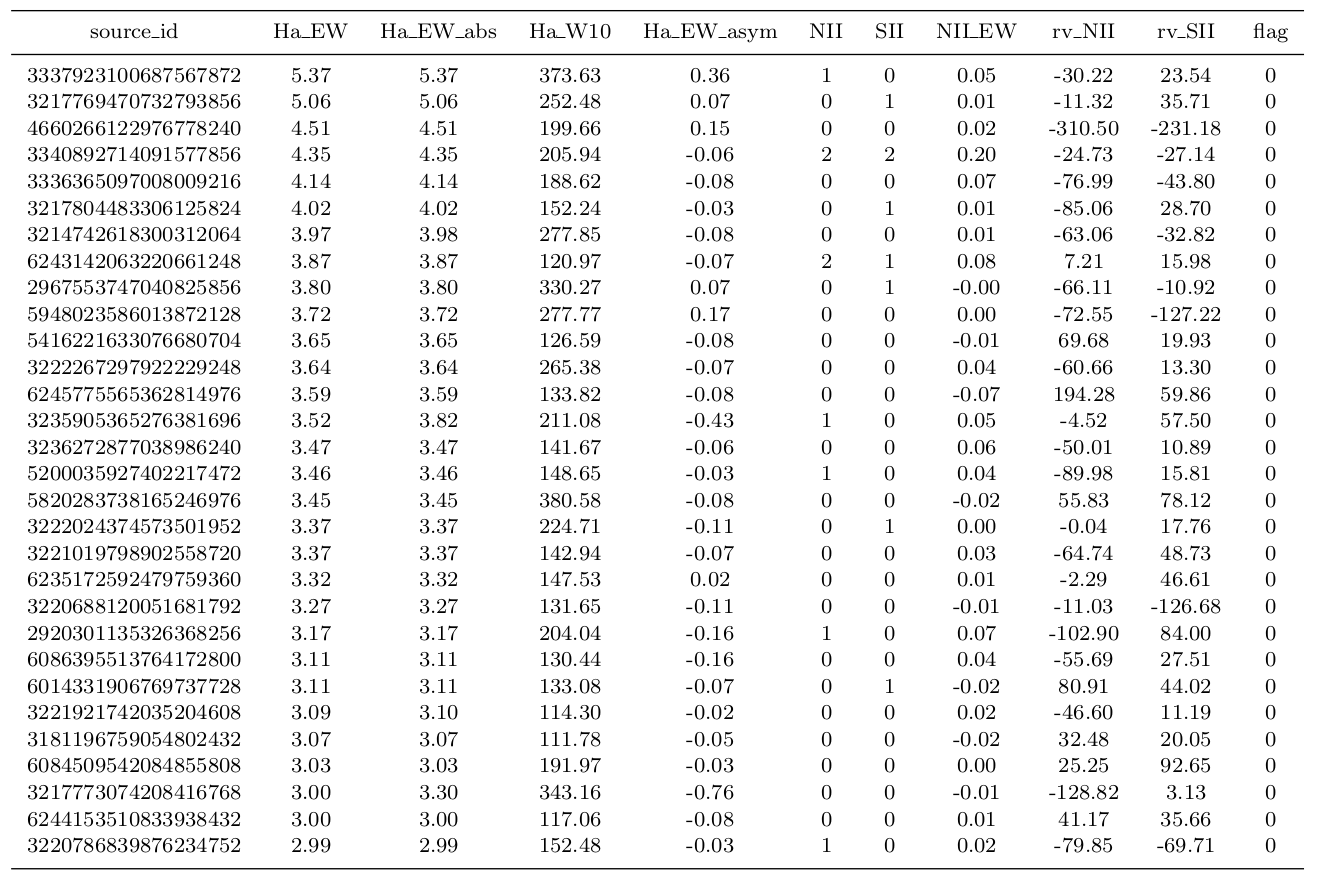
\includegraphics[scale=.40]{figures/cotartable.png}
\caption{The 30 strongest emitters. Reproduced from Čotar et al. (2021)\cite{vcotar2021galah}}
\end{figure}
